\cleardoublepage
\newpage
\ifdefined\EnableIncludeImages
    \ThisULCornerWallPaper{1.0}{chapterimage.eps}
\fi
\chapter{Zorra}

%Zorra era plomo blanco morochas o chispiado
%Zandor nace 1961 (probablemente)
%%Zandor nace 1961 cuando yo tenía aprox 5-6 años

\ifdefined\EnableIncludeImages
\begin{wrapfigure}{r}{0.49\textwidth}
  \begin{center}
  \vspace{-30pt}
    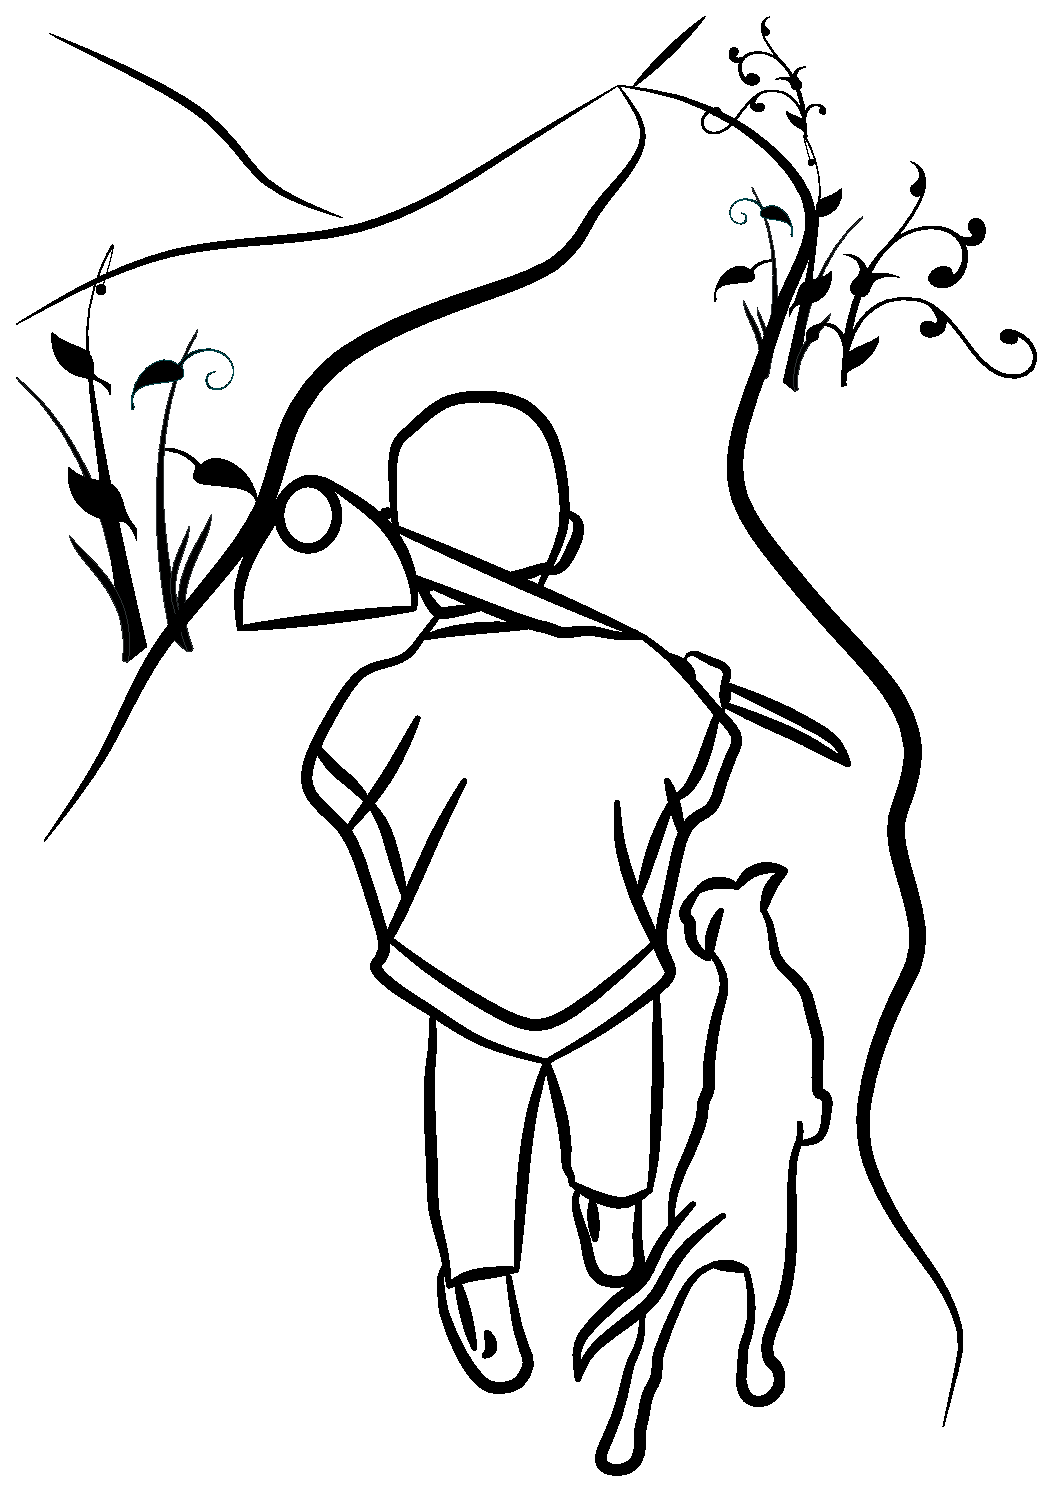
\includegraphics[width=0.47\textwidth]{caminhando.eps}
  \end{center}
  \vspace{-20pt}
  %\caption{Zandor}
\end{wrapfigure}
\fi
Cuando era niño, mi familia tenía una perra que se llamaba Zorra, ella era de carácter gentil y muy amorosa con todos nosotros; a mi papá y a mí nos gustaba andar con ella para todos lados. En algunas ocasiones, durante nuestras caminatas, nosotros avistábamos a algún conocido o familiar, y ellos se dirigían a mi padre diciendo a viva voz:\\\indent
--- Buenos días Don Juande!\\\indent
El respondía entusiasmado a esos saludos con la misma alegría y energía.
Mi padre en verdad se llamaba Juan de Dios; sin embargo, cariñosamente, todas las personas del pueblo preferían llamarlo Don Juande.

Yo probablemente tendría cinco o seis años en esa época y recuerdo de forma clara cómo mi perra iba corriendo de forma ágil delante de nosotros, ladrando contenta abriéndonos camino a través de los montes.
Estas caminatas eran muy comunes, dado que teníamos que llevar comida a las vacas, buscarlas cuando alguna se perdía, o hacer algún tipo de mantenimiento a la chacra.
Al principio yo no percibí que mi perra tenia algunas malas costumbres, pues con ella nosotros convivíamos y andábamos de día, y su comportamiento era irreprochable.

\ifdefined\EnableIncludeImages
\begin{wrapfigure}{r}{0.42\textwidth}
  \begin{center}
  \vspace{-30pt}
    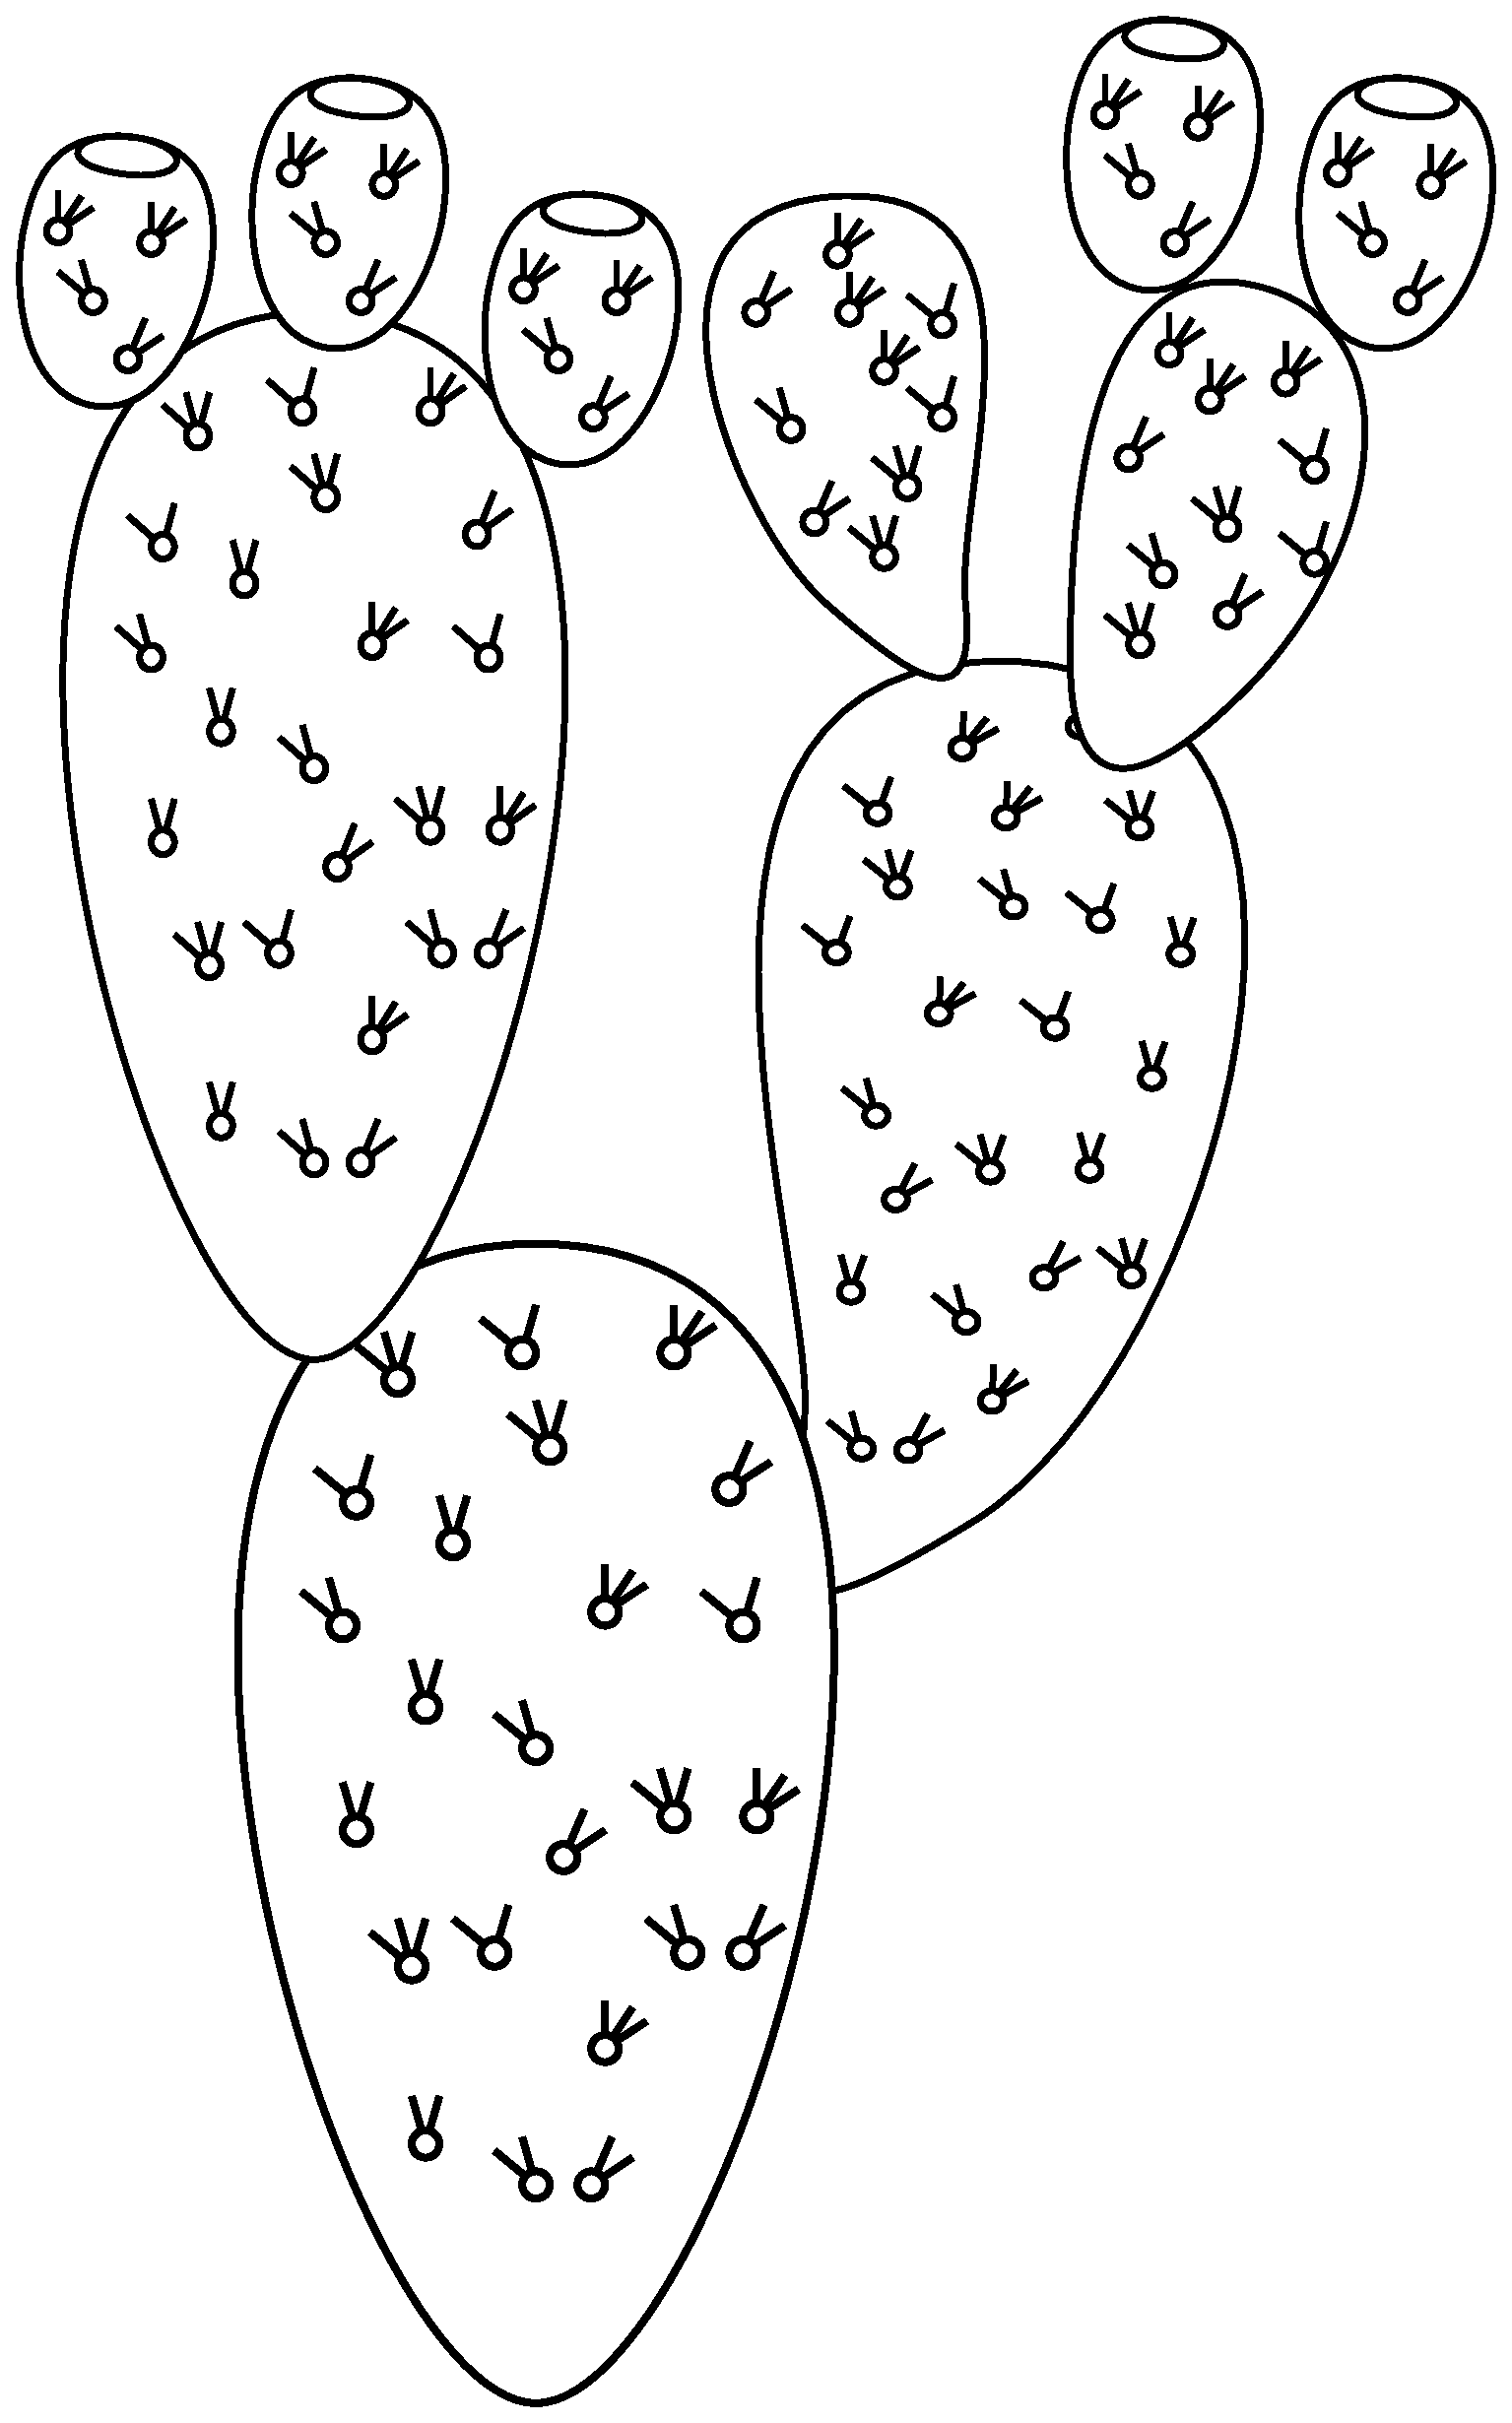
\includegraphics[width=0.3\textwidth]{opuntia.eps}
  \end{center}
  \vspace{-20pt}
  %\caption{Figo das índias.}
\end{wrapfigure}
\fi
Aun recuerdo la primera vez que fui al río acompañando a mi papá y a Zorra. Mi mamá le había encargado, con carácter de urgencia, la misión de obtener pescados para freírlos en el almuerzo; yo rápidamente me uní a tan noble encomienda, pues me gustaba salir a andar.
Para llegar al río, nosotros tuvimos que bajar por una ladera a través de un camino cercado por plantas de tuna. Cuando llegamos allá, vi que el margen de las aguas estaba lleno de carrizos, siendo ese un lugar óptimo para explorar y jugar. Así, en cuanto mi papá pescaba, mi perra y yo buscábamos nidos con huevos de perdiz, sin embargo, Zorra siempre los encontraba primero, comía todo, o casi todo, y yo solamente conseguía salvar algunos para mí. 

De esa forma pasaron algunos años, en los cuales nadie llegó a nuestra casa trayendo quejas o comentarios sobre Zorra; sin embargo, un día entré a la huerta que estaba cerca a mi casa y quedé sorprendido al encontrar varios pequeños ``tesoros'' dentro de un escondite. Había una saco de tela con pan, otro con azúcar, uno con dulces y algunas pequeñas herramientas sueltas.
Para mi todo eso era increíble, pues nosotros solo teníamos cosas como azúcar o galletas cuando mi papá regresaba de sus viajes después de trabajar cuatro meses en Ica o en alguna otra ciudad grande. 
En un primer momento, la alegría invadió mi corazón, sin embargo, recordé que mi papá era una persona muy rigurosa, no le gustaba tomar las cosas de los demás, y decía: \\\indent
--- Si tu encuentras alguna cosa en el camino, en el campo o en la pampa, no lo debes tomar ---
y él agregaba:
--- Seguramente alguien lo dejó caer, la persona que lo perdió va a regresar a buscarlo, y si tú te lo llevas, no lo va a encontrar.

Yo recordaba muy bien esa enseñanza, porque una vez, cuando yo estaba en la soledad del campo pastando mis vacas, encontré una herramienta para hacer hilos de lana, que en mi pueblo llamamos ``callapa''\footnote{También llamado huso, este es um utensilio cilíndrico hecho generalmente de madera, utilizado para hilar y retorcer fibras como la lana.}; probablemente la herramienta era de algún otro pastor que pasó por allí, mas en aquel momento no pensé en eso, solo tomé la callapa y retorné a mi casa; ya en la tarde, llegué muy contento, diciendo:\\\indent
--- Mamá, papá, miren lo que encontré en el campo!\\\indent
Mi papá inmediatamente respondió:  
--- Aquí no hay nada para ser encontrado! Eso es de alguien, alguna persona lo há perdido y ella va a volver a buscarlo. Vuelve y deja eso donde lo encontraste.

\ifdefined\EnableIncludeImages
\begin{wrapfigure}{r}{0.42\textwidth}
  \begin{center}
  \vspace{-10pt}
    
\includegraphics[width=0.4\textwidth]{tools-spindle.eps}
  \end{center}
  \vspace{-20pt}
  %\caption{Figo das índias.}
\end{wrapfigure}
\fi
En ese momento un frío pasó desde la punta de mi cabeza hasta las puntas de mis pies, pues ya casi eran las seis de la tarde, todo estaba obscuro, las pocas luces eran muy lejanas y solamente venían de las casas de los vecinos --- esto era así porque en la sierra, en esa época, las familias vivían en casas a unos 200, 300, 400 metros de distancia o, a veces, incluso más ---, y para finalizar, yo era muy miedoso en lo que se refiere a lugares obscuros y donde tenia que ir estaba muy lejos.

Delante de la orden de mi padre, yo fui corriendo y llorando en aquella dirección. En el camino no podía distinguir las cosas a unos metros de mí, porque la luna estaba menguante; entretanto, cuando estaba casi a la mitad de mi destino y mi caminar era cada vez mas vacilante, observé las sombras a mi alrededor, y en un sendero paralelo al mio, entre piedras y arboles grandes, vi la silueta de mi papá siguiéndome a escondidas y a una distancia significativa.
Con esa certeza en mi corazón, yo seguí mi camino con un poco mas de tranquilidad, pues sentía que mi papá me estaba cuidando; aun así, yo seguía llorando de miedo, porque en la sierra, la noche es densa y absoluta, y los sonidos del camino alimentaban fácilmente la imaginación de un niño.
En el último tercio del camino, yo decidí ir corriendo, ya que sentía que no podía aguantar más esa situación. Por fin, llegué a mi destino, tiré la callapa en el exacto lugar donde la había encontrado y rápidamente emprendí el camino de retorno.
Al volver, también sentí la presencia de mi papá a algunos metros de mí, o por lo menos yo quería creer eso. Con esa seguridad llegué a mi casa en menos tiempo del que gasté para ir, sin embargo, cuando entré, mi papá estaba sentado allí como si nada hubiese sucedido.

Por esa vieja experiencia, y teniendo la seguridad de la autoría de Zorra, ya que ese escondite era su lugar favorito, yo tuve mucho miedo por ella, pues sabia que a mi papá no le gustaría que Zorra estuviera tomando cosas de otras personas; por lo que, si yo le avisaba, mi papá la castigaría severamente. Por ese motivo decidí no decir nada sobre mi descubrimiento, entretanto, tengo que reconocer que: además del amor a mi perra, también pesó en mi decisión que el lugar estuviera lleno de azúcar, pan y otras cosas, que para nosotros, gente de la sierra, eran considerados lujos.
Por ese motivo decidí pasar por allí antes de ir a la escuela o a la chacra: para comer galletas, agua con azúcar o cualquier otra cosa deliciosa que estuviera allí.
Para mi desesperación, un día Zorra trajo demasiadas cosas, yo no podía imaginar de donde había tomado todo eso, ya que ella solo ``trabajaba'' durante la noche, mientras todos dormíamos. Así, delante de aquel aumento en los robos que largamente desbordaba su escondite, mi papá descubrió toda la situación.
Muy a mi pesar, él la castigó severamente, desde mi casa yo solamente escuché sus lamentos recibiendo la punición, pues preferí no ver.


Después de esa experiencia, ella dejó de llevar las cosas a la huerta, y el problema parecía resuelto. No obstante, luego descubriríamos que lejos de casa, en una piedra grande y obscura, cerca de la casa de un vecino, 
Zorra había reiniciado sus actividades. Así, de día, delante de los ojos de la familia, se comportaba como una perra ejemplar. Sin embargo, durante la noche, ella robaba de los vecinos las mas variadas cosas.

\ifdefined\EnableIncludeImages
\begin{wrapfigure}{r}{0.42\textwidth}
  \begin{center}
  \vspace{-10pt}
    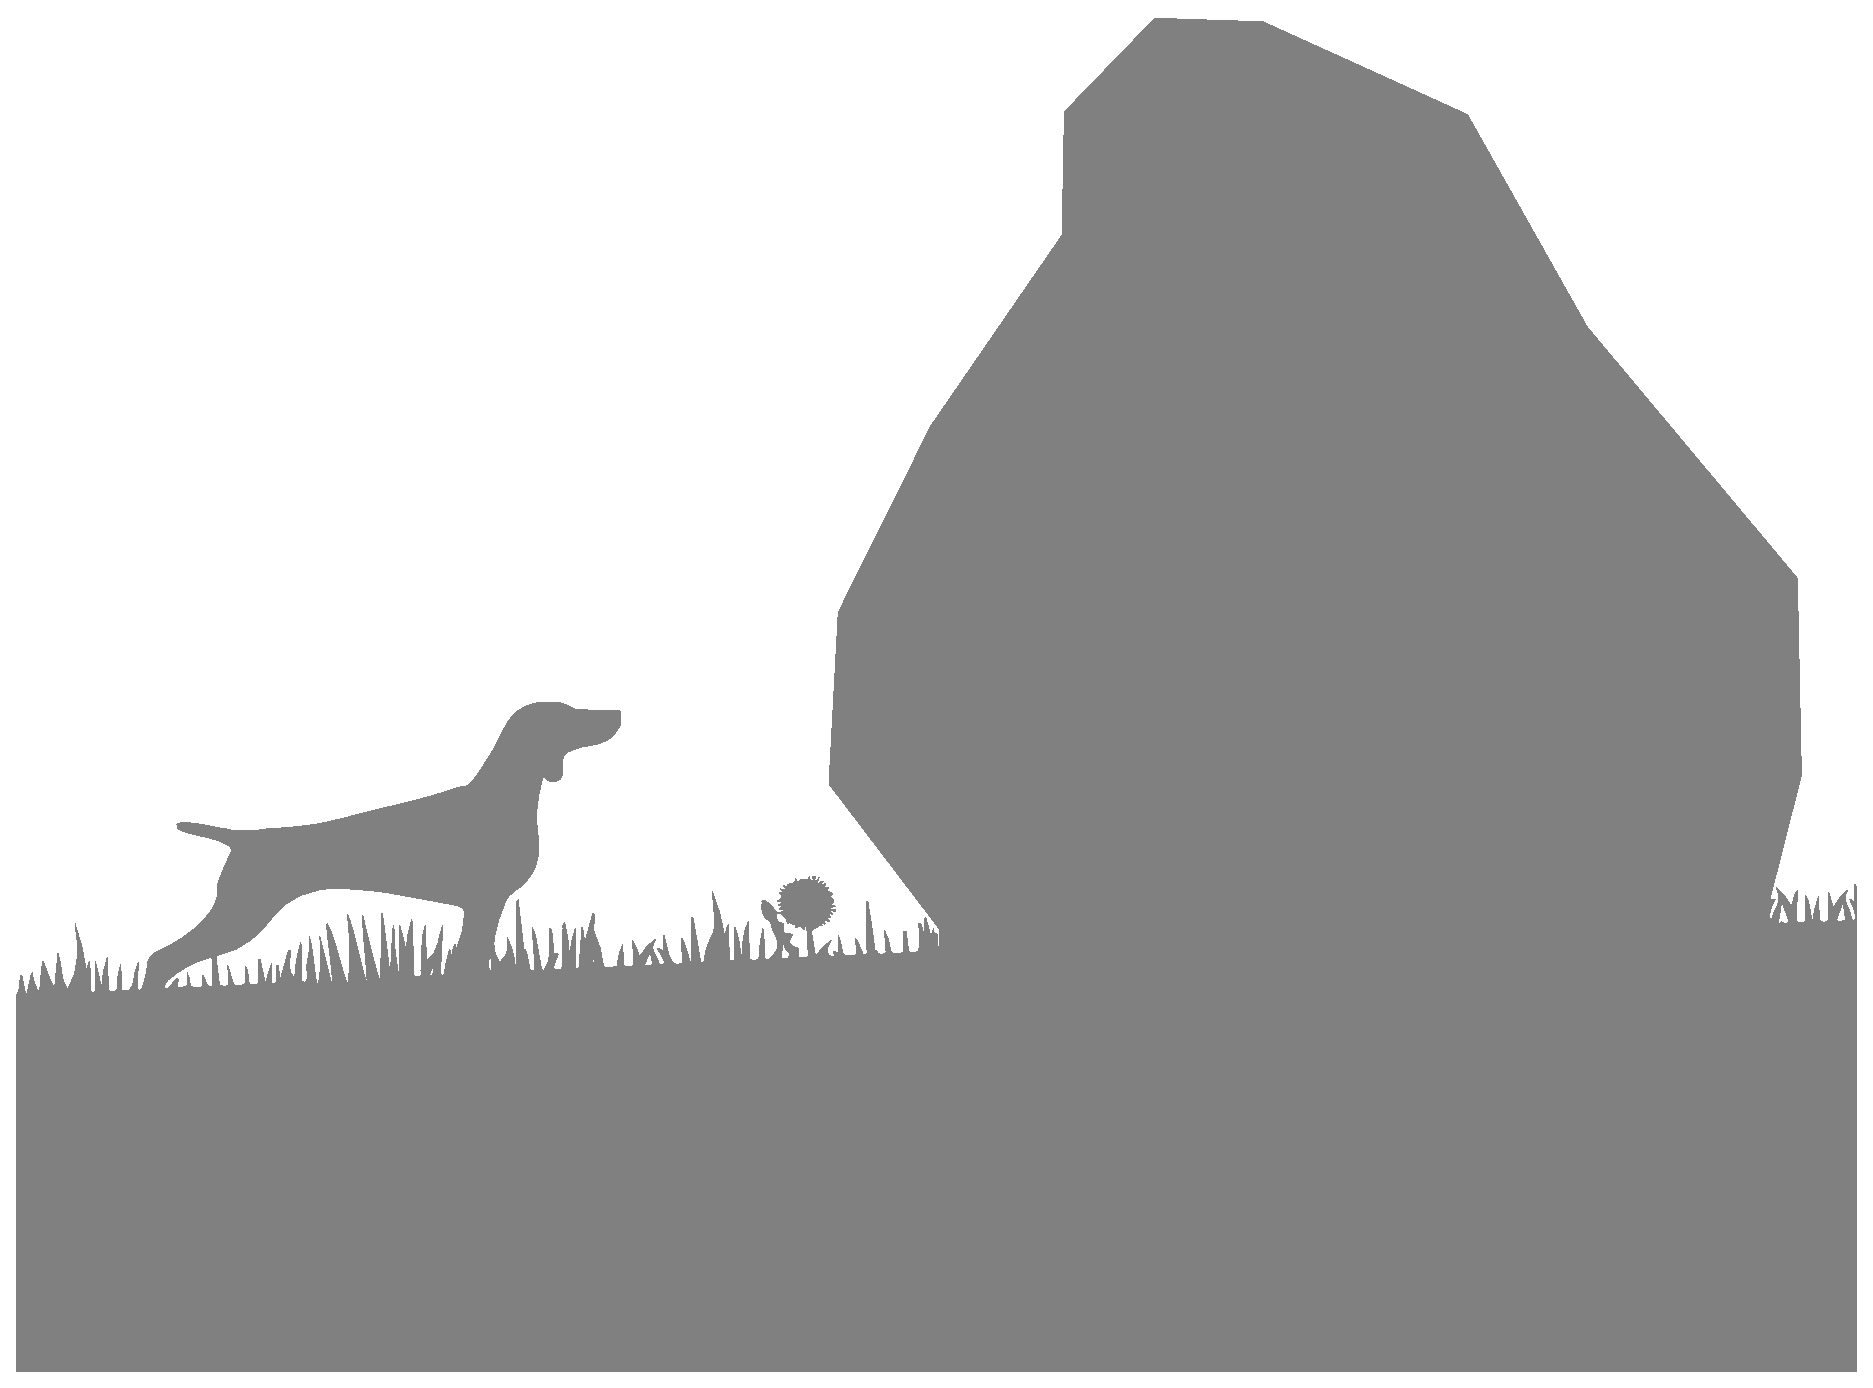
\includegraphics[width=0.4\textwidth]{zorra-rock.eps}
  \end{center}
  \vspace{-20pt}
  %\caption{Figo das índias.}
\end{wrapfigure}
\fi
En ese momento fue la primera vez que una persona llegó a mi casa para hacer una reclamación. El agraviado denunció que vio personalmente como Zorra había entrado a su casa para robar.
La indignación de mi papá fue tan grande como su vergüenza, pues no fue un vecino o algún familiar nuestro, que podría entender la situación, sino que fue una víctima que vivía muy lejos de nosotros, en otro pueblo, que fue preguntando entre los vecinos hasta encontrar primero sus cosas y luego nuestra casa.
En esa ocasión mi papá castigó mas severamente a Zorra; delante de esa difícil situación, mi mayor tristeza era que yo ya comprendía que ese problema no iba a solucionarse con otro castigo, y mis dudas fueron confirmadas cuando percibí que Zorra seguía saliendo de noche.

Mucho tiempo después descubriríamos que Zorra nuevamente había cambiado de escondite y que llevaba sus cosas a otra piedra grande, cerca de la casa de una vecina que era viuda y que cariñosamente llamábamos abuela Misla --- en verdad, ella no era familiar nuestro, mas la costumbre en la sierra era llamar abuela a cualquier persona de edad, como señal de respeto, ya que vivíamos con ellos como si fuesen de nuestra familia ---.
Así, antes de que alguna persona de mi casa conociese ese nuevo lugar, en el cual Zorra ocultaba sus objetos robados, otra persona llegó a denunciar nuevamente a la perra, y aun cuando que mi papá castigó, gritó e intentó seguirla, no conseguimos encontrar el nuevo escondite. Así, el tiempo pasó sin que esa incógnita fuese resuelta.

Un día mi papá decidió bajar al río para pescar, dado que yo era andariego me apresuré a acompañarlo junto con Zorra. 
%no encontramos a Zorra para que nos acompañe.
Cuando llegamos allá me divertí mucho jugando en el agua y ayudando a mi papá, así pasó el día y cuando eran las cuatro o cinco de la tarde, nosotros estábamos listos para regresar a casa con la pesca del día.
En ese momento percibí la ausencia de Zorra y inicié a llamarla para que nos acompañe, 
sin embargo, en cuanto la estaba buscando, escuché un ruido entre los carrizos del río, donde yo acostumbraba jugar con Zorra, por pura curiosidad fui a averiguar que era ese sonido similar a un llanto agudo. Para mi sorpresa, allí estaba solitario un cachorro pequeño y negrito que mi perra había parido.
Hasta ese momento yo no había percibido que mi perra estaba embarazada, solamente pensé que estaba un poco gordita,
pero rápidamente entendí la situación
Para que mi papá no lo viera, yo escondí al cachorro dentro de mi chompa, ya que desconfiaba que él me dejase llevar un nuevo perro a casa, pues los problemas que Zorra generaba ya eran suficientes para nosotros, como para arriesgar más la reputación de la familia con otro perro.
Así, después de encontrar a Zorra volvimos a casa, yo con el corazón en la mano por la emcoión.
Solo cuando llegué a casa saqué al perro de dentro de mis ropas y delante de mis hermanas, mi mamá y mi papá, presenté al nuevo miembro de la familia. Dado que en aquella época, mis hermanas estaban aprendiendo a leer usando un libro llamado ``Lola y Pepe'', donde en sus historias describían a un perro llamado Zandor, yo decidí usar ese nombre para mi nuevo perro.

Así, aun con sus nuevos deberes de mamá, Zorra no dejaba de causar problemas, ya que a nuestros oídos llegaban historias de robos en pueblos distantes, y las ausencias de Zorra se volvían cada vez más prolongadas.
Para nuestra mala suerte, en un pueblo vecino, se había expandido la noticia que era una perra la responsable de todos los robos, y, en un triste día, los moradores de esa localidad se organizaron, entre todos consiguieron acorralarla y atraparla, y finalmente, sobre el abrigo de la multitud y sin ningún remordimiento, dieron muerte a mi querida Zorra. 
Ese mismo día llegó a mi casa la noticia de su muerte... entre lágrimas y lamentos fuimos a ese pueblo para enterrar a nuestra querida perra, ya que nos informaron que ellos simplemente habían tirado su cuerpo en la ribera del río. Cuando llegamos allá, la encontramos helada e inerte, e instintivamente la envolvimos en un paño, como si fuese un bebé, para que no pasase frío... a su lado lloramos hasta que nuestras lágrimas se secaron, pues ella había sido nuestra amiga fiel, y aunque supiéramos de sus malas costumbres, nosotros la amábamos.
En ese mismo lugar, al finalizar el día y con el río como testigo, hicimos una pequeña ceremonia y enterramos a quien en vida fue conocida por nosotros como Zorra.

Al día siguiente, la noticia ya se había esparcido en mi pueblo, y aunque nosotros asumíamos que no recibiríamos condolencias por parte de los vecinos, para nuestro desengaño, la abuela Misla llegó llorando a la puerta de nuestra casa y entre sus lamentos decía:
\begin{quotation}
\noindent ``Yo no tenía olla, y \\Zorra me llevó una olla;\\ 
yo no tenía sartén, y \\Zorra me llevó una sartén;\\ 
yo no tenía cuchara, y \\Zorra me llevó una cuchara;\\
yo no tenía cuchillo, y \\Zorra me llevó un cuchillo;\\
cuando tuve hambre, \\Zorra me llevó pan...''
\end{quotation}
Mi mamá la abrazaba, en cuanto la abuela Misla continuaba con su letanía, por aquel animal que, a su modo de ver, solo había llegado a su vida para ayudarla en su momento de mayor necesidad.

